\section{Introduction to Rendering}
Il \textbf{Rendering} è il processo che converte i dati in input in immagini.
Paradigmi del Rendering:
\begin{itemize}
    \item Ray Tracing
    \item Path Tracing
    \item Rasterization-based Pipeline
\end{itemize}
per visualizzare scene 3D abbiamo bisogno di trasformale in immagini sintetiche che possono essere mostrate sullo schermo.
Esistono diversi algoritmi per trasformare una scena 3D in una raster image, in seguito veranno presentati due algoritmi appartenenti a due famiglie differenti:
\begin{itemize}
    \item Ray tracing algorithms
    \item Rasterization-based algorithms
\end{itemize} 
\subsection{Pinhole Camera}
La metafora usata per descrivere la relazione tra l'osservatore e la scena è quella della camera virtuale
Per convenzione, assumiamo l'esistenza di un piano immagine tra la scena e il centro di proiezione.
\begin{figure}[H]
    \centering
    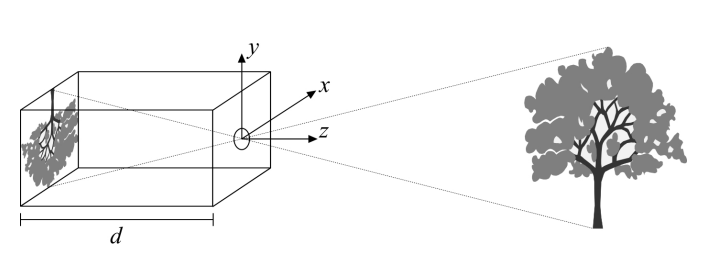
\includegraphics[width=0.5\textwidth]{images/PinHole.png} 
    \caption{Pinhole camera}
    \label{fig:immagine}
\end{figure}
La fotocamera virtuale consiste in un parallelepipedo nel quale la faccia anteriore ha un foro infinitesimale (fotocamera a foro stenopeico) e sul retro vengono formate le immagini; l'angolo $\theta$ di visualizzazione può essere modificato variando il rapporto tra la distanza focale d e la dimensione h del piano immagine.
\subsubsection{Perspective Projection}
\begin{figure}[H]
    \centering
    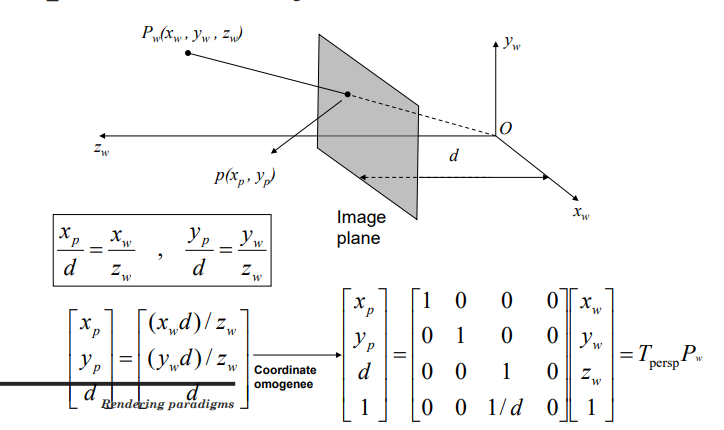
\includegraphics[width=0.5\textwidth]{images/PerspPro.png} 
    \caption{Prospective Projection}
    \label{fig:immagine}
\end{figure}
così possiamo scrivere \\
$\begin{bmatrix}
    x_p \\
    y_p \\
    1      
\end{bmatrix}=
\begin{bmatrix}
    1 & 0 & 0 & 0 \\
    0 & 1 & 0 & 0 \\
    0& 0 & 1/d & 0 \\   
\end{bmatrix}  
\begin{bmatrix}
    x_w \\
    y_w \\
    z_w  \\
    1  
\end{bmatrix}   $
\\ o in maniera equivalente: \\
$\begin{bmatrix}
    x_p \\
    y_p \\
    1      
\end{bmatrix}= K[I|0]P_w  \ \ \ 
K=\begin{bmatrix}
    d & 0 & 0 \\
    0 & d & 0 \\
    0 & 0 & 1  \\
\end{bmatrix} P_w$
\subsubsection{From image plane to pixel coordinates}
\begin{figure}[H]
    \centering
    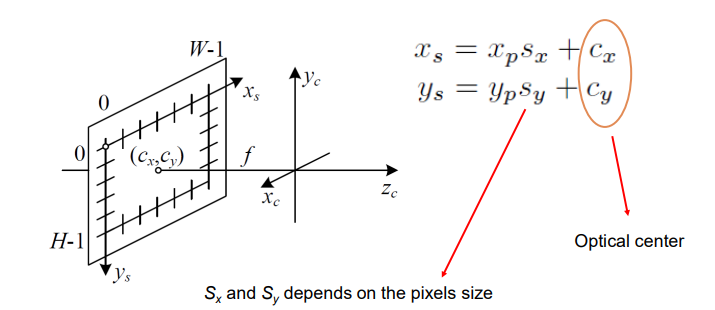
\includegraphics[width=0.5\textwidth]{images/fromto.png} 
    \caption{To pixel coordinates}
    \label{fig:immagine}
\end{figure}
\subsubsection{Camera Model}
$\begin{bmatrix}
    x_p \\
    y_p \\
    1      
\end{bmatrix}= K[I|0]P_w $
\\ Calibration matrix, von $f_{sx} e y facla lenght$: \\
$K= \begin{bmatrix}
    f_{sx}  & s & c_x \\
    0 & f_{sy} & c_y \\
    0 & 0 & 1      
\end{bmatrix}P_w$ \\
Versione Usuale: \\
$K= \begin{bmatrix}
    f  & 0 & c_x \\
    0 & f & c_y \\
    0 & 0 & 1      
\end{bmatrix}P_w$
\\ Prendendo in considerazione la posizione a l'orientamento della camera nella scena: \\
$\begin{bmatrix}
    x_p \\
    y_p \\
    1      
\end{bmatrix}= K[I|0]MP_w $
 \ \ \
 M=$\begin{bmatrix}
    R & t \\
    1 & 0  
\end{bmatrix}$
\\
$p_s più \ o \ meno PP_w$  \\
Quindi, abbiamo due insiemi di parametri che caratterizzano la fotocamera.
\begin{itemize}
    \item \textbf{Parametri intrinseci}: lunghezza focale, dimensione dei pixel, risoluzione, centro ottico.
    \item \textbf{Parametri estrinseci}: posizione e orientamento della fotocamera, cioè una rotazione e una traslazione.
\end{itemize}
\subsection{Ray-Tracing}
Idea principale: tracciare i raggi luminosi all'indietro
Per ogni pixel dello schermo:
  \begin{itemize}
    \item Sparare un raggio (chiamato raggio primario)
    \item Trovare l'intersezione con la primitiva più vicina.
  \end{itemize}
Il nucleo è: l'intersezione raggio/primitiva (deve essere estremamente ottimizzata).
Facile da gestire: riflessioni speculari multiple, facile da realizzare: semitrasparenza con rifrazioni, facile da gestire: ombre (nitide).
\begin{figure}[H]
    \centering
    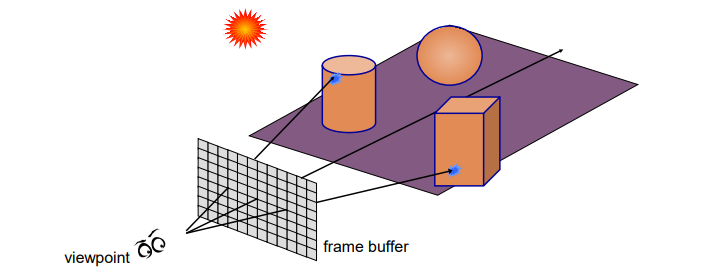
\includegraphics[width=0.5\textwidth]{images/RayTraces.png} 
    \caption{Ray-Tracing}
    \label{fig:immagine}
\end{figure}
\textbf{Pseudocodice}
\begin{algorithm}[H]
    \SetAlgoLined
    \KwResult{Color the pixels on the screen}
    \For{each pixel in the screen}{
        Generate a primary ray from the camera's viewpoint through the pixel\;
        
        Find the closest intersection between the ray and objects in the scene\;
        
        \If{an intersection exists}{
            Calculate the color at the intersection point considering material properties, lights, and illumination\;
            
            If needed, cast further rays (secondary rays) for effects like shadows, reflections, refractions\;
            
            Combine the computed colors via secondary ray intersections with the main color\;
            
            Assign the resulting color to the pixel on the screen\;
        }
        \Else{
            Assign a background color to the pixel\;
        }
    }
    \caption{Pseudocode for Basic Ray Tracing}
    \end{algorithm}
    \begin{figure}[H]
        \centering
        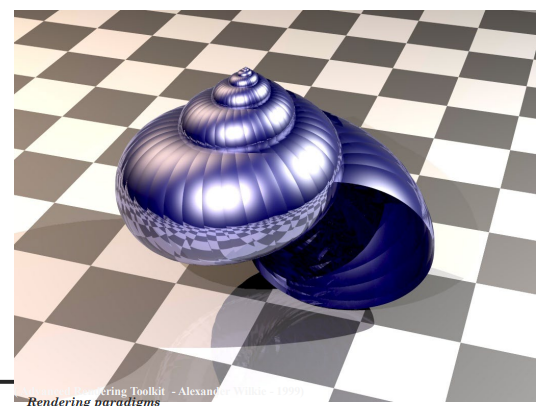
\includegraphics[width=0.5\textwidth]{images/ExRayTrace.png} 
        \caption{ Esempio di Ray-Tracing}
        \label{fig:immagine}
    \end{figure}
    \begin{itemize}
        \item \textbf{Nucleo principale}:
        \begin{itemize}
            \item Calcolo dell'intersezione tra un \textbf{RAGGIO 3D} e \textbf{PRIMITIVI 3D}
        \end{itemize}
        \item Computazionalmente complesso:
        \begin{itemize}
            \item Elevato costo
            \item Tuttavia SUBLINEARE! (rispetto al conteggio delle primitive)
        \end{itemize}
        \item Se si utilizzano le strutture corrette: \textbf{indicizzazione spaziale}!
        \item L'indicizzazione spaziale sono un insieme di strutture dati speciali (gerarchiche, basate sull'hashing) per accelerare il calcolo dell'intersezione raggio/scena.
        \item Una volta utilizzate solo per elaborazioni offline:
        \begin{itemize}
            \item Ora in tempo reale nei casi più semplici sfruttando le GPU
        \end{itemize}
    \end{itemize}
    \subsection{Rasterization-Based Rendering}
    
La rasterizzazione è il processo di conversione di oggetti o immagini descritte in forma vettoriale o geometrica in una griglia regolare di pixel su uno schermo o un dispositivo di visualizzazione. Questo processo è utilizzato per rappresentare graficamente oggetti o immagini su schermi bidimensionali, come monitor, televisori o dispositivi mobili.

In sostanza, la rasterizzazione prende informazioni continue o vettoriali e le traduce in informazioni discrete su una griglia di pixel. Ad esempio, in grafica 3D, gli oggetti tridimensionali vengono proiettati su una vista bidimensionale e successivamente convertiti in pixel attraverso la rasterizzazione per essere visualizzati su uno schermo.
    \begin{minipage}{0.45\textwidth}
        \begin{algorithm}[H]
        \SetAlgoLined
        \ForEach{pixel $p$}{
            Make a ray $r$\;
            \ForEach{primitive $o$ in scene}{
                \If{intersect($r$, $o$)}{
                    Find color for $o$\;
                    Color $p$ with it\;
                }
            }
        }
        \caption{Algorithm 1: Ray-Tracing}
        \end{algorithm}
        \end{minipage}
        \hfill
        \begin{minipage}{0.45\textwidth}
        \begin{algorithm}[H]
        \SetAlgoLined
        \ForEach{primitive $o$}{
            Find where $o$ falls on screen\;
            Rasterize 2D shape\;
            \ForEach{produced pixel $p$}{
                Find color for $o$\;
                Color $p$ with it\;
            }
        }
        \caption{Algorithm 2: Rasterization}
        \end{algorithm}
        \end{minipage}
\textbf{Trasformazioni}:
\begin{itemize}
    \item Trasformazioni dei sistemi di coordinate
    \item Obiettivo: proiettare le primitive nello spazio dello schermo
    \item ... ma anche assemblare le primitive per comporre la scena
\end{itemize}
\textbf{Illuminazione}:
\begin{itemize}
    \item Calcolo dell'illuminazione
    \item Obiettivo: calcolare il colore finale di ogni parte della scena
    \item Per fare ciò dobbiamo considerare:
    \begin{itemize}
        \item Caratteristiche ottiche
        \item Illuminazione della scena
        \item Geometria degli oggetti
    \end{itemize}
\end{itemize}
Dato che l'hardware grafico è ottimizzato per rasterizzare triangoli, l'intera scena viene decomposta in TRIANGOLI tridimensionali
\begin{figure}[H]
    \centering
    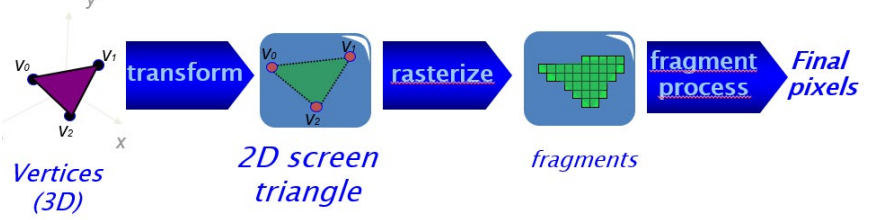
\includegraphics[width=0.5\textwidth]{images/RasterProcess.png} 
    \caption{Rasterization-Based Rendering}
    \label{fig:immagine}
\end{figure}
Input: insieme di vertici e i loro attributi associati \\
\begin{itemize}
    \item L'algoritmo passa attraverso diverse fasi:
    \begin{enumerate}
        \item Trasformazioni per vertice e configurazione degli attributi
        \item Elaborazione delle primitive
        \item Rasterizzazione
        \item Calcolo per frammento
    \end{enumerate}
\end{itemize}
\subsection(Rasterization vs Ray-Tracing)
\begin{figure}[H]
    \centering
    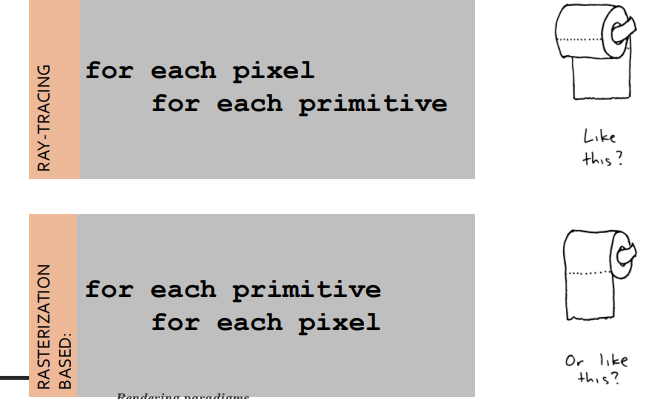
\includegraphics[width=0.5\textwidth]{images/RayvsRed.png} 
    \caption{Rendering Algoorithms Paradigms}
    \label{fig:immagine}
\end{figure}
Vantaggi del \textbf{Ray-Tracing}:
\begin{itemize}
    \item buono per complessi effetti visuali
    \item Algoritmo concettualmente semplice
    \item Considera gli effetti GLOBALI
    \item Rappresentazione più realistica degli effetti luminosi
    \item Maggiore libertà delle primitive (è più semplice intersecare che proiettare e rasterizzare)
    \item Potenzialmente grande scalabilità con la complessità della scena
\end{itemize}
Vantaggi della \textbf{Rasterization}:

\begin{itemize}
    \item veolce, per ogni primitiva vengono processati solo alcuni pixels!
    \item Più facilmente parallelizzabile?
    \item Complessità più controllabile
    \item Più adatto alle schede grafiche (per ora)
    \item Più semplice con dati dinamici?
    \item Migliore gestione dell'anti-aliasing (più avanti)
    \item Migliore scalabilità con la risoluzione dell'immagine
\end{itemize}
\subsubsection{Visione Storica}
\textbf{Ray-tracing}
\begin{itemize}
    \item Algoritmo di scelta per il rendering OFFLINE
    \item Utilizzato per FILM (e immagini statiche CGI)
    \item Preferito da Pixar, Dreamworks, ecc.
    \item Noti ray-tracer: POV-ray, RenderMan, YafaRay...
\end{itemize}

\textbf{Rasterization}
\begin{itemize}
    \item Algoritmo di scelta per il rendering in TEMPO REALE
    \item Utilizzato per GIOCHI (e anteprime, e 3D sul web...)
    \item Preferito da Nvidia, ATI, ecc.
    \item Primo a ottenere hardware specializzato
\end{itemize}
\subsubsection{Reality}
Non necessariamente LENTO!
\begin{itemize}
    \item Algoritmi e strutture dati per "query spaziali" efficienti
    \item Anche sub-lineare rispetto al numero di primitive!
\end{itemize}
.. non necessariamente SOLO software:
\begin{itemize}
    \item Hardware specializzato?
    \item Progetto OpenRT
    \item Tecnologie di tracciamento dei raggi in tempo reale inTrace GmbH
    \item MPI Informatik, Saarbrueken - Ingo Wald 2004 Paradigmi di rendering 50
\end{itemize}

\begin{itemize}
    \item ..non necessariamente priva di effetti visivi complessi (anzi, richiedono solo alcune approssimazioni e alcuni algoritmi avanzati)
\end{itemize}
            




